%%%%%%%%%%%%%%%%%%%%%%%%%%%%%%%%%%%%%%%%%%%%%%%%%%%%%%%%%%%%%%%%%%%%%%%%%%%%%%%%%%%%%%%%%%%%%%%%%%%%%%%%%%%%%%%%%%%%%%%%%%%%%%%%%%%%%%%%%%%%%%%%%%%%%%%%%%%%%%%%%%%%%%%%%%%%%%%%%%%%%%%%%%%%
% Written By Michael Brodskiy
% Class: AP Chemistry
% Professor: J. Morgan
%%%%%%%%%%%%%%%%%%%%%%%%%%%%%%%%%%%%%%%%%%%%%%%%%%%%%%%%%%%%%%%%%%%%%%%%%%%%%%%%%%%%%%%%%%%%%%%%%%%%%%%%%%%%%%%%%%%%%%%%%%%%%%%%%%%%%%%%%%%%%%%%%%%%%%%%%%%%%%%%%%%%%%%%%%%%%%%%%%%%%%%%%%%%

\documentclass[12pt]{article} 
\usepackage{alphalph}
\usepackage[utf8]{inputenc}
\usepackage[russian,english]{babel}
\usepackage{titling}
\usepackage{amsmath}
\usepackage{graphicx}
\usepackage{enumitem}
\usepackage{amssymb}
\usepackage[super]{nth}
\usepackage{expl3}
\usepackage[version=4]{mhchem}
\usepackage{hpstatement}
\usepackage{rsphrase}
\usepackage{everysel}
\usepackage{ragged2e}
\usepackage{geometry}
\usepackage{fancyhdr}
\usepackage{cancel}
\usepackage{siunitx}
\usepackage{chemfig}
\geometry{top=1.0in,bottom=1.0in,left=1.0in,right=1.0in}
\newcommand{\subtitle}[1]{%
  \posttitle{%
    \par\end{center}
    \begin{center}\large#1\end{center}
    \vskip0.5em}%

}
\newcommand{\orbital}[2]{{%
    \def\+{\big|\hspace{-2pt}\overline{\underline{\hspace{2pt}\upharpoonleft}}}%
    \def\-{\overline{\underline{\downharpoonright\hspace{2pt}}}\hspace{-2pt}\big|}%
    \def\0{\big|\hspace{-2pt}\overline{\underline{\phantom{\hspace{2pt}\downharpoonright}}}}%
    \def\1{\overline{\underline{\phantom{\downharpoonright\hspace{2pt}}}}\hspace{-2pt}\big|}%
  \setlength\tabcolsep{0pt}% remove extra horizontal space from tabular
  \begin{tabular}{c}$#2$\\[2pt]#1\end{tabular}%
}}
\DeclareSIUnit\Molar{\textsc{m}}
\DeclareSIUnit\atm{\textsc{atm}}
\DeclareSIUnit\torr{\textsc{torr}}
\DeclareSIUnit\psi{\textsc{psi}}
\DeclareSIUnit\bar{\textsc{bar}}
\DeclareSIUnit\Celsius{\textsc{C}}
\usepackage{hyperref}
\hypersetup{
colorlinks=true,
linkcolor=blue,
filecolor=magenta,      
urlcolor=blue,
citecolor=blue,
}

\urlstyle{same}


\title{Chapter 14 $-$ Equilibrium with Acid/Base Reactions}
\date{\today}
\author{Michael Brodskiy\\ \small Instructor: Mr. Morgan}

% Mathematical Operations:

% Sum: $$\sum_{n=a}^{b} f(x) $$
% Integral: $$\int_{lower}^{upper} f(x) dx$$
% Limit: $$\lim_{x\to\infty} f(x)$$

\begin{document}

\maketitle

\begin{itemize}

  \item Buffered Solutions $-$ Resist pH change. Made of weak acid and concentrated base.

    \begin{enumerate}

      \item  Ex. \ce{HC2H3O2} and \ce{NaC2H3O2}. Add: \ce{HCl} and \ce{NaOH}

    \end{enumerate}

  \item Buffer Capacity $-$ How many ions can be added to destroy the buffers effectiveness

  \item Titration $-$ Adding an acid to base or base to acid to determine concentration

  \item When the amount of acid-base is at the equivalence point, $M_aV_a=M_bV_b$

    \begin{enumerate}

      \item Indicators are used to tell if the solution is at an equivalence point

    \end{enumerate}

  \item Three main indicators:
    
    \begin{enumerate}

      \item Methyl Red $-$ End point = 5. Acid is red, base is yellow.
        
      \item Bromothymol Blue $-$ End point = 7. Acid is yellow, base is blue

      \item Phenolphalein $-$ End point = 9. Acid is colorless, base is pink

    \end{enumerate}

  \item End point needs to coincide with the equivalence point

  \item Titration Curve for Strong and Strong

    \begin{center}
      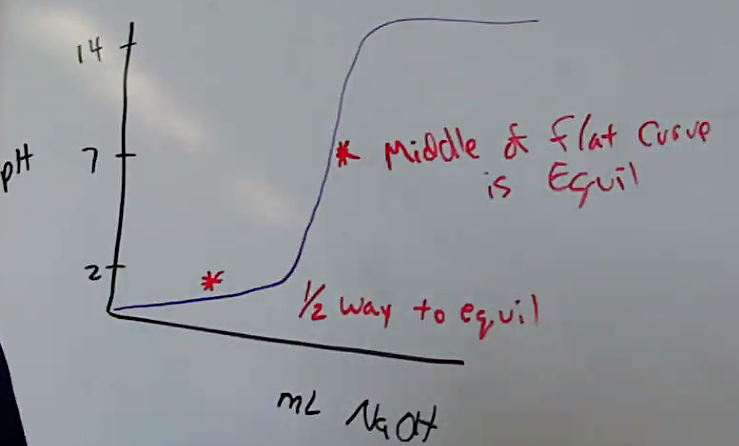
\includegraphics[width=.8\textwidth]{Figures/TitrationCurveSS.png}\\
      Titration Curve Example
    \end{center}

\end{itemize}

\end{document}

